\documentclass[11pt]{beamer}
\title{SVMRanker: A General Termination Analysis Framework of Loop Programs via SVM}
\usepackage{verbatim}
\usepackage{amsmath}
\usepackage{amsthm}
\usepackage{listings}
\usepackage{graphics}
\usepackage{color}
\usepackage{stmaryrd}
\usepackage{multicol}
\usepackage{tabularx}
\usepackage{listings}
\usepackage{tikz}

\usetikzlibrary{automata,shapes,arrows,patterns,calc,positioning}
\tikzset{every picture/.style={->, >=stealth', shorten >=0pt, auto, initial text={}}}
\tikzstyle{flowchartelement} = [draw, inner sep=3pt, align=center]
\tikzstyle{inputoutput} = [flowchartelement, trapezium, trapezium right angle=-70pt, trapezium left angle=70pt]
\tikzstyle{test} = [flowchartelement, diamond]
\tikzstyle{code} = [flowchartelement, minimum width=20mm, rectangle]
\tikzstyle{connector} = [draw, circle, fill=black, inner sep=1.25pt]
\newtheorem{proposition}{Proposition}
\author{
    Authors: \textbf{Xie Li}, Yi Li, Yong Li, Xuechao Sun \\Andrea Turrini and Lijun Zhang
}
\date{\today}


\begin{document}
\maketitle

\begin{frame}[fragile]\frametitle{Verification}
Checking termination is neccessary.
\begin{example}
\begin{minipage}{\linewidth}
\begin{lstlisting}[language=C++,
    xleftmargin=.3\textwidth, 
    xrightmargin=.3\textwidth]
assume(True);
int x = 1;
while(x>0) x++;
assertion(x<=0);
\end{lstlisting}
\end{minipage}
\end{example}
The assertion can be checked once the loop is terminating.


However theoretically...

In the practice the program return \texttt{UNKNOWN} once we cannot prove or disprove the termination.

Our tool: focus on the synthesis ranking function.

What is \textbf{ranking function}?
\end{frame}



\begin{frame}[fragile]\frametitle{Ranking Function}
\begin{multicols}{2}
\begin{minipage}{\linewidth}

\texttt{assume(True);}\\
\texttt{int x = 5;}\\
\texttt{while(x > 0) x--;}\\
\texttt{assertion(x<=0);}\\
\end{minipage}

ranking function is the function used for proof of termiation.
\[\Omega(\mathbf{x}, \mathbf{x}') := x > 0 \wedge x' = x - 1 \]
Ranking function: 
\[f(\mathbf{x}) = x\]

\begin{itemize}
\item Informally: $f: S\rightarrow \mathbb{R}$ where $S$ is the set of states and $\mathbb{R}$ is a well-founded ordered set.

\item strictly decreases at each iteration.

\item has a lower bound in the loop state space.

\end{itemize}

\end{multicols}
\end{frame}

\begin{frame}\frametitle{More Powerful Ranking Functions}
\begin{itemize}
\item Linear ranking function: $f(\mathbf{x}) = \mathbf{ax} + b$.
\item Polynomial ranking function.
\item $k$-phase- nested or multiphase ranking function:
\[\langle f_1, \cdots, f_k\rangle\]
\end{itemize}

\end{frame}

\begin{frame}\frametitle{Synthesis of Ranking Function}

\begin{itemize}
\item Prove the termination is UNDECIDABLE.
\item Synthesis of a certain class of ranking function is DECIDABLE.
\end{itemize}

\end{frame}

\begin{frame}\frametitle{State-of-the-Art Tools}
Termination problem is essential and basic to program verification.

State-of-the-art tools:
\begin{itemize}
\item \textsc{LassoRanker} in \textsc{Ultimate Automizer}.
\item \textsc{iRankFinder}: A tool for ranking function inferring.
\item \textsc{Loopster}: A static loop termination analyzer.
\item \textsc{CPAChecker}
\item ...
\end{itemize}
Competition \textsc{SV-COMP} also has a termination track for this problem.

\end{frame}



\begin{frame}\frametitle{\textsc{SVMRanker}: Synthesize Ranking Function via SVM}
\begin{center}

Technique previous tools use.
\end{center}

\begin{center}
We reduce the synthesis of ranking functions
\\ into the SVM problem.
\end{center}

\begin{center}
Advantage? Disadvantage?
\end{center}


\end{frame}

\begin{frame}\frametitle{SVMRanker: Architecture}
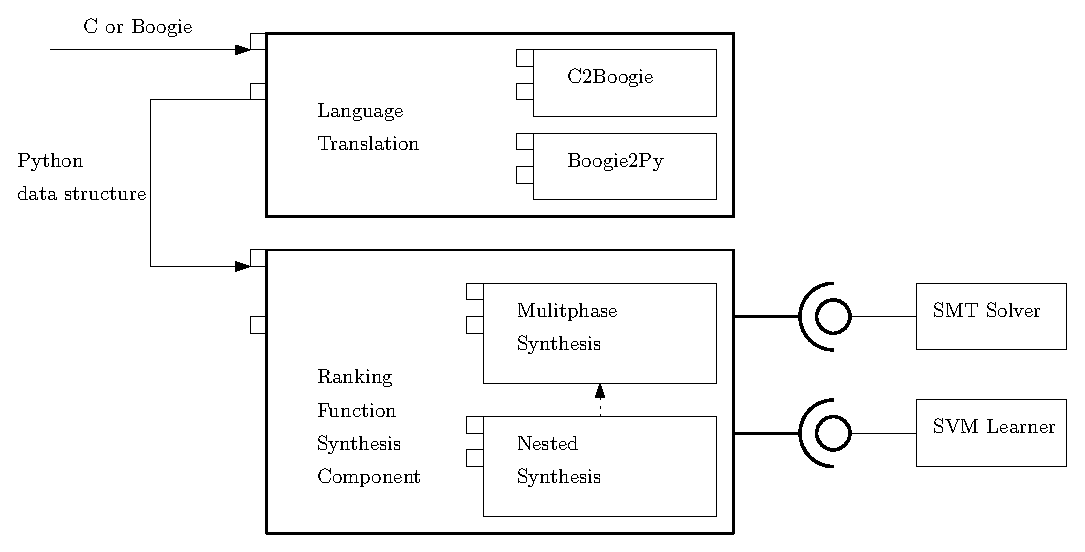
\includegraphics[scale=0.65]{archi1.eps}
\end{frame}

\begin{frame}\frametitle{Experimental Results: Nonlinear Loops}
Cases are adapted from \textsc{SV-COMP}.
\begin{table}
\tiny
	\label{tab:nonlinear}
	\centering
	\begin{tabular}{c|c|c|c|c}
	Case ID & \textsc{SVMRanker} & \textsc{iRankFinder} & \textsc{LassoRanker} & \textsc{CPAChecker}\\
	\hline 
	116 & U &U& U & U \\
	148 & Y &U& U & F\\
	149 & Y &U& U & U\\
	151 & Y &U& U & F\\
	152 & Y &U& U & F\\
	153 & Y &U& U & F\\
	154 & U &U& U & F\\
	155 & Y &U& U & F\\
	157 & Y &U& U & U\\
	158 & Y &U& U & TO \\
	159 & Y &U& U & F\\
	160 & Y &U& U & TO\\
	161 & U &U& U & F\\
	162 & Y &U& U & F\\
	163 & Y &U& U & F\\
	164 & Y &U& U & U\\
	167 & Y &U& U & E\\
	171 & Y &U& U & E\\
	DoubleNeg & U&U & U & U
	\end{tabular}
\end{table}
\end{frame}

\begin{frame}\frametitle{Experimental Results: Linear Loops}
\end{frame}
\end{document}